\documentclass{article}[18pt]
\usepackage{../../../../format}
\lhead{Networks and Systems - Security}


\begin{document}
\begin{center}
\underline{\huge Software Security}
\end{center}
\section{Types of memory}
\begin{defin}[DRAM]
1 Transistor per bit
\begin{itemize}
	\item "slow"
	\item cheap
\end{itemize}
\end{defin}

\begin{defin}[SRAM]
	4+ transistors per bit
	\begin{itemize}
		\item fast ($\sim$ 4 clock cycles)
		\item expensive
		\item Takes up space on die
	\end{itemize}
\end{defin}
\section{Computer Architecture}
\begin{center}
	\includegraphics[width=0.7\linewidth]{"Computer Architecture"}
\end{center}
\section{GPU}
\textbf{GDDR5} is "slow" and cheap
\section{The Stack}
\begin{center}
	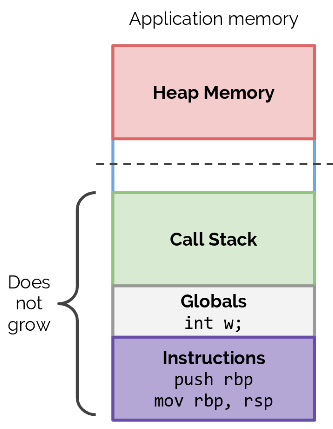
\includegraphics[scale=0.4]{stack}
\end{center}
\begin{itemize}
	\item When a program thread starts, the operating system reserves some amount of space for the stack - stack memory does not grow during runtime
\end{itemize}
The stack being full is cased by
\begin{itemize}
	\item Badly written recursive functions
	\item Too much local memory allocated (especially with multi-threading)
\end{itemize}
\section{The Heap}
\begin{center}
	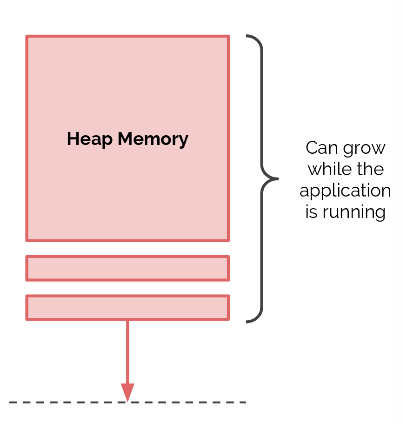
\includegraphics[scale=0.7]{heap}
\end{center}
\begin{itemize}
	\item Memory is not guaranteed to be initialised to zero
	\item Can malloc memory to same size of some sensitive data
\end{itemize}
\section{Understanding the platform}
\begin{itemize}
	\item The key to writing good, secure software is to understand the platform
	\item Hardware is the base platform (for software)
	\item Lots of things get in the way
\end{itemize}

\end{document}